\documentclass[11pt, a4paper]{article}

% Fonts and Encoding
\usepackage[utf8]{inputenc}
\usepackage[T1]{fontenc}

% Math and Symbols
\usepackage{amsmath, amssymb, amsthm, amsfonts, mathrsfs, mathtools}

% Layout and Geometry
\usepackage{geometry}
\geometry{a4paper, margin=1in}

% Formatting and Graphics
\usepackage{graphicx, xcolor, enumitem, booktabs, array, tabularx}

% TikZ for Illustrations
\usepackage{tikz}
\usetikzlibrary{arrows.meta, positioning, shapes.geometric, calc, backgrounds}

% Clickable Links and TOC
\usepackage{hyperref}
\hypersetup{
    colorlinks=true,
    linkcolor=blue,
    filecolor=magenta,      
    urlcolor=cyan,
    pdftitle={Advanced Continuous Probability Distributions},
}

% Theorem Environments
\newtheorem{theorem}{Theorem}[section]
\newtheorem{lemma}[theorem]{Lemma}
\newtheorem{proposition}[theorem]{Proposition}
\newtheorem{corollary}[theorem]{Corollary}
\theoremstyle{definition}
\newtheorem{definition}{Definition}[section]
\newtheorem{axiom}{Axiom}[section]
\newtheorem{example}{Example}[section]
\theoremstyle{remark}
\newtheorem{remark}{Remark}[section]

% Custom Commands
\newcommand{\R}{\mathbb{R}}
\newcommand{\N}{\mathbb{N}}
\newcommand{\Z}{\mathbb{Z}}
\newcommand{\Q}{\mathbb{Q}}
\newcommand{\E}{\mathbb{E}}
\newcommand{\Prob}{\mathbb{P}}
\newcommand{\F}{\mathcal{F}}

\title{\textbf{Advanced Continuous Probability Distributions: \\ Measure-Theoretic Foundations and Applications}}
\author{Tashfeen Omran}
\date{\today}

\begin{document}

\maketitle
\tableofcontents
\newpage

\section{Part 1: Comprehensive Introduction, Context, and Prerequisites}

\subsection{Core Concepts and Axioms}
In the rigorous study of probability theory, we transition from discrete counting arguments to the continuous domain using the framework of measure theory. A probability space is formally defined as a triplet $(\Omega, \F, \Prob)$, where $\Omega$ is the sample space, $\F$ is a $\sigma$-algebra of measurable events, and $\Prob$ is a probability measure satisfying Kolmogorov's Axioms. 

A continuous random variable $X$ is a measurable function $X: \Omega \to \R$. Unlike discrete variables, the probability of a continuous random variable taking any single exact value is zero, i.e., $\Prob(X = x) = 0$. Instead, probabilities are assigned to intervals via the Lebesgue integral of a non-negative, Lebesgue-measurable function called the Probability Density Function (PDF), denoted $f(x)$. The fundamental axiom linking the PDF to the probability measure is:
\[ \Prob(a \le X \le b) = \int_{a}^{b} f(x) \, dx \]

\subsection{Intuition and Set-Theoretic Foundations}
Intuitively, a random variable acts as a bridge, mapping abstract outcomes $\omega \in \Omega$ to the real number line $\R$. The probability measure $\Prob$ on $\Omega$ induces a new measure $\Prob_X$ on $\R$, known as the pushforward measure. The PDF $f(x)$ can be viewed as the Radon-Nikodym derivative of this induced measure with respect to the standard Lebesgue measure. 

In this document, we focus on two foundational continuous distributions:
\begin{itemize}
    \item \textbf{The Uniform Distribution:} Represents the principle of indifference. Mass is spread evenly across an interval $[a, b]$. It is the continuous analog of equally likely outcomes.
    \item \textbf{The Normal (Gaussian) Distribution:} The cornerstone of probability, characterized by its symmetric, bell-shaped curve. It arises naturally from the sum of independent random variables.
\end{itemize}

\subsection{Historical Context and Motivation}
The formalization of continuous probability was driven by the need to model physical measurements and astronomical errors in the 18th and 19th centuries. Carl Friedrich Gauss and Pierre-Simon Laplace independently derived the Normal distribution to model measurement errors, leading to the Central Limit Theorem. Later, in the 1930s, Andrey Kolmogorov unified these applied concepts under the rigorous umbrella of measure theory, resolving foundational crises regarding the definition of continuous randomness.

\subsection{Key Theorems and Formulas}
\begin{theorem}[Law of the Unconscious Statistician - LOTUS]
If $X$ is a continuous random variable with PDF $f(x)$ and $g: \R \to \R$ is a measurable function, the expected value of $g(X)$ is given by:
\[ \E[g(X)] = \int_{-\infty}^{\infty} g(x) f(x) \, dx \]
\end{theorem}

\begin{theorem}[Standardization of Normal Variables]
If $X \sim \mathcal{N}(\mu, \sigma^2)$, then the affine transformation $Z = \frac{X - \mu}{\sigma}$ results in a standard normal random variable $Z \sim \mathcal{N}(0, 1)$.
\end{theorem}

\subsection{Prerequisites}
To fully grasp the proofs in this document, the reader must be proficient in:
\begin{itemize}
    \item \textbf{Real Analysis:} Riemann and Lebesgue integration, improper integrals, and the Fundamental Theorem of Calculus.
    \item \textbf{Set Theory:} Operations on sets, intersections, unions, and subsets.
    \item \textbf{Differential Calculus:} The chain rule, product rule, and optimization techniques (first and second derivative tests).
\end{itemize}

\newpage
\section{Part 2: Detailed Homework Solutions}

\subsection{Problem 4.38: Uniform Cumulative Distribution}
\textbf{Problem:} Suppose that $Y$ has a uniform distribution over the interval $(0, 1)$.
\textbf{a)} Find $F(y)$.
\textbf{b)} Show that $\Prob(a \le Y \le a + b)$, for $a \ge 0, b \ge 0$, and $a + b \le 1$ depends only upon the value of $b$.

\textbf{Solution a):}
\textit{Proof Technique: Direct Integration.}
By definition, the probability density function (PDF) of $Y \sim \mathcal{U}(0,1)$ is:
\[ f(y) = \begin{cases} 1, & 0 \le y \le 1 \\ 0, & \text{elsewhere} \end{cases} \]
The cumulative distribution function (CDF), $F(y)$, is defined as $F(y) = \int_{-\infty}^{y} f(t) \, dt$. We evaluate this integral across three distinct regions of $\R$:
\begin{itemize}
    \item \textbf{Case 1 ($y < 0$):} 
    \[ F(y) = \int_{-\infty}^{y} 0 \, dt = 0 \]
    \item \textbf{Case 2 ($0 \le y \le 1$):} 
    \[ F(y) = \int_{-\infty}^{0} 0 \, dt + \int_{0}^{y} 1 \, dt = 0 + [t]_{0}^{y} = y \]
    \item \textbf{Case 3 ($y > 1$):} 
    \[ F(y) = \int_{-\infty}^{0} 0 \, dt + \int_{0}^{1} 1 \, dt + \int_{1}^{y} 0 \, dt = 0 + 1 + 0 = 1 \]
\end{itemize}
Thus, the CDF is rigorously defined as:
\[ F(y) = \begin{cases} 0, & y < 0 \\ y, & 0 \le y \le 1 \\ 1, & y > 1 \end{cases} \]
$\blacksquare$

\textbf{Solution b):}
\textit{Proof Technique: Direct Algebraic Substitution.}
We are given $a \ge 0, b \ge 0$, and $a + b \le 1$. This implies that both $a$ and $a+b$ lie strictly within the interval $[0, 1]$.
Using the fundamental property of the CDF, the probability of $Y$ falling in an interval is:
\[ \Prob(a \le Y \le a + b) = F(a + b) - F(a) \]
Since both arguments are in $[0, 1]$, we use the branch $F(y) = y$:
\[ \Prob(a \le Y \le a + b) = (a + b) - a = b \]
This result is exactly $b$, which is independent of $a$. Thus, the probability depends only on the interval length $b$.
$\blacksquare$

\subsection{Problem 4.43: Transformation of a Uniform Variable}
\textbf{Problem:} A circle of radius $r$ has area $A = \pi r^2$. If a random circle has a radius that is uniformly distributed on the interval $(0, 1)$, what are the mean and variance of the area of the circle?

\textbf{Solution:}
\textit{Proof Technique: Law of the Unconscious Statistician (LOTUS) and Moment Computation.}
Let $R \sim \mathcal{U}(0,1)$. The PDF of $R$ is $f(r) = 1$ for $r \in (0,1)$ and $0$ elsewhere.
The area is a random variable defined by the non-linear transformation $A = \pi R^2$.
To find the mean $\E[A]$, we apply LOTUS:
\[ \E[A] = \E[\pi R^2] = \int_{-\infty}^{\infty} \pi r^2 f(r) \, dr \]
\[ \E[A] = \int_{0}^{1} \pi r^2 (1) \, dr = \pi \left[ \frac{r^3}{3} \right]_{0}^{1} = \frac{\pi}{3} \]
To find the variance, we use the identity $\text{Var}(A) = \E[A^2] - (\E[A])^2$.
First, we compute the second moment $\E[A^2]$:
\[ \E[A^2] = \E[(\pi R^2)^2] = \E[\pi^2 R^4] = \int_{0}^{1} \pi^2 r^4 (1) \, dr \]
\[ \E[A^2] = \pi^2 \left[ \frac{r^5}{5} \right]_{0}^{1} = \frac{\pi^2}{5} \]
Now, substitute into the variance formula:
\[ \text{Var}(A) = \frac{\pi^2}{5} - \left( \frac{\pi}{3} \right)^2 = \frac{\pi^2}{5} - \frac{\pi^2}{9} = \pi^2 \left( \frac{9 - 5}{45} \right) = \frac{4\pi^2}{45} \]
\textbf{Final Answer:} The mean area is $\frac{\pi}{3}$ and the variance is $\frac{4\pi^2}{45}$.
$\blacksquare$

\subsection{Problem 4.53: Poisson Processes and Uniform Conditioning}
\textbf{Problem:} The number of defective circuit boards coming off a soldering machine follows a Poisson distribution. During a specific eight-hour day, one defective circuit board was found.
\textbf{a)} Find the probability that it was produced during the first hour.
\textbf{b)} Find the probability that it was produced during the last hour.
\textbf{c)} Given that no defective boards were produced during the first four hours, find the probability that the defective board was manufactured during the fifth hour.

\textbf{Solution:}
\textit{Proof Technique: Conditional Probability and Poisson Process Properties.}
A fundamental theorem of Poisson processes states that if exactly $n$ events occur in an interval $[0, t]$, the exact times of these occurrences are distributed as the order statistics of $n$ independent uniform random variables on $[0, t]$.
Here, $n = 1$ event occurred in the interval $[0, 8]$. Let $Y$ be the time the defective board was produced. Therefore, $Y \sim \mathcal{U}(0, 8)$.
The PDF of $Y$ is $f(y) = \frac{1}{8}$ for $y \in [0, 8]$.

\textbf{Part a):} The first hour corresponds to the interval $[0, 1]$.
\[ \Prob(0 \le Y \le 1) = \int_{0}^{1} \frac{1}{8} \, dy = \left[ \frac{y}{8} \right]_{0}^{1} = \frac{1}{8} \]

\textbf{Part b):} The last hour corresponds to the interval $[7, 8]$.
\[ \Prob(7 \le Y \le 8) = \int_{7}^{8} \frac{1}{8} \, dy = \left[ \frac{y}{8} \right]_{7}^{8} = \frac{8 - 7}{8} = \frac{1}{8} \]

\textbf{Part c):} We are given the condition that no defects occurred in the first four hours, meaning $Y > 4$. We want to find the probability that the defect occurred in the fifth hour, meaning $4 \le Y \le 5$.
Using the definition of conditional probability:
\[ \Prob(4 \le Y \le 5 \mid Y > 4) = \frac{\Prob(4 \le Y \le 5 \cap Y > 4)}{\Prob(Y > 4)} \]
Since the event $\{4 \le Y \le 5\}$ is a strict subset of $\{Y > 4\}$, their intersection is simply $\{4 \le Y \le 5\}$.
\[ \Prob(4 \le Y \le 5) = \int_{4}^{5} \frac{1}{8} \, dy = \frac{1}{8} \]
\[ \Prob(Y > 4) = \int_{4}^{8} \frac{1}{8} \, dy = \frac{4}{8} = \frac{1}{2} \]
Therefore:
\[ \Prob(4 \le Y \le 5 \mid Y > 4) = \frac{1/8}{1/2} = \frac{2}{8} = \frac{1}{4} \]
$\blacksquare$

\subsection{Problem 4.70: Normal Distribution and Binomial Trials}
\textbf{Problem:} GPAs are normally distributed with mean 2.4 and standard deviation 0.8. Suppose that three students are randomly selected. What is the probability that all three will possess a GPA in excess of 3.0?

\textbf{Solution:}
\textit{Proof Technique: Standardization of Normal Variables and Independence.}
Let $Y$ be the GPA of a randomly selected student. We are given $Y \sim \mathcal{N}(2.4, 0.8^2)$.
First, we find the probability that a single student has a GPA greater than 3.0, i.e., $\Prob(Y > 3.0)$.
We standardize $Y$ by subtracting the mean $\mu$ and dividing by the standard deviation $\sigma$ to create a standard normal variable $Z \sim \mathcal{N}(0,1)$:
\[ \Prob(Y > 3.0) = \Prob\left( \frac{Y - 2.4}{0.8} > \frac{3.0 - 2.4}{0.8} \right) = \Prob\left( Z > \frac{0.6}{0.8} \right) = \Prob(Z > 0.75) \]
Using standard normal distribution properties:
\[ \Prob(Z > 0.75) = 1 - \Prob(Z \le 0.75) \approx 1 - 0.7734 = 0.2266 \]
Let $p = 0.2266$ be the probability of success for a single student.
Since the three students are selected randomly, their GPAs are independent events. Let $X$ be the number of students out of 3 who have a GPA $> 3.0$. Then $X \sim \text{Binomial}(3, p)$.
We want the probability that all three have a GPA $> 3.0$, which is $\Prob(X = 3)$:
\[ \Prob(X = 3) = \binom{3}{3} p^3 (1-p)^0 = p^3 = (0.2266)^3 \]
\[ (0.2266)^3 \approx 0.0116 \]
\textbf{Final Answer:} The probability is approximately $0.0116$ (or $1.16\%$).
$\blacksquare$

\subsection{Problem 4.79: Inflection Points of the Normal Density}
\textbf{Problem:} Show that the normal density with parameters $\mu$ and $\sigma$ has inflection points at the values $\mu - \sigma$ and $\mu + \sigma$.

\textbf{Solution:}
\textit{Proof Technique: Differential Calculus (First and Second Derivatives).}
The probability density function of a normal distribution is:
\[ f(y) = \frac{1}{\sigma\sqrt{2\pi}} \exp\left( -\frac{(y-\mu)^2}{2\sigma^2} \right) \]
An inflection point occurs where the second derivative $f''(y)$ changes sign, which requires $f''(y) = 0$.
First, we compute the first derivative $f'(y)$ using the chain rule:
\[ f'(y) = \frac{1}{\sigma\sqrt{2\pi}} \exp\left( -\frac{(y-\mu)^2}{2\sigma^2} \right) \cdot \frac{d}{dy} \left( -\frac{(y-\mu)^2}{2\sigma^2} \right) \]
\[ f'(y) = f(y) \cdot \left( -\frac{2(y-\mu)}{2\sigma^2} \right) = -f(y) \frac{y-\mu}{\sigma^2} \]
Next, we compute the second derivative $f''(y)$ using the product rule:
\[ f''(y) = \frac{d}{dy} \left[ -f(y) \frac{y-\mu}{\sigma^2} \right] = - \left[ f'(y) \frac{y-\mu}{\sigma^2} + f(y) \frac{d}{dy} \left( \frac{y-\mu}{\sigma^2} \right) \right] \]
\[ f''(y) = - \left[ \left( -f(y) \frac{y-\mu}{\sigma^2} \right) \frac{y-\mu}{\sigma^2} + f(y) \frac{1}{\sigma^2} \right] \]
Factor out $f(y)$:
\[ f''(y) = f(y) \left[ \frac{(y-\mu)^2}{\sigma^4} - \frac{1}{\sigma^2} \right] \]
To find the inflection points, we set $f''(y) = 0$. Since the exponential function $f(y)$ is strictly positive for all $y \in \R$, we must have:
\[ \frac{(y-\mu)^2}{\sigma^4} - \frac{1}{\sigma^2} = 0 \implies \frac{(y-\mu)^2}{\sigma^4} = \frac{1}{\sigma^2} \]
Multiply both sides by $\sigma^4$:
\[ (y-\mu)^2 = \sigma^2 \]
Taking the square root of both sides yields:
\[ y - \mu = \pm \sigma \implies y = \mu \pm \sigma \]
Since the term $\frac{(y-\mu)^2}{\sigma^4} - \frac{1}{\sigma^2}$ changes sign from positive to negative at $y = \mu - \sigma$ and from negative to positive at $y = \mu + \sigma$, the concavity of the curve changes at these points. Thus, $y = \mu - \sigma$ and $y = \mu + \sigma$ are indeed inflection points.
$\blacksquare$

\subsection{Problem 4.80: Expectation of a Function of a Normal Variable}
\textbf{Problem:} Assume that $Y$ is normally distributed with mean $\mu$ and standard deviation $\sigma$. After observing a value of $Y$, a mathematician constructs a rectangle with length $L = |Y|$ and width $W = 3|Y|$. Let $A$ denote the area of the resulting rectangle. What is $\E[A]$?

\textbf{Solution:}
\textit{Proof Technique: Expectation of a Function of a Random Variable.}
We are given $Y \sim \mathcal{N}(\mu, \sigma^2)$.
The area of the rectangle is given by $A = L \times W = |Y| \times 3|Y| = 3|Y|^2 = 3Y^2$.
We need to find the expected value of $A$:
\[ \E[A] = \E[3Y^2] \]
By the linearity of expectation, we can factor out the constant:
\[ \E[A] = 3\E[Y^2] \]
To find the second moment $\E[Y^2]$, we use the fundamental definition of variance:
\[ \text{Var}(Y) = \E[Y^2] - (\E[Y])^2 \]
We know that for $Y \sim \mathcal{N}(\mu, \sigma^2)$, the variance is $\text{Var}(Y) = \sigma^2$ and the mean is $\E[Y] = \mu$. Substituting these known values:
\[ \sigma^2 = \E[Y^2] - \mu^2 \]
Rearranging to solve for $\E[Y^2]$:
\[ \E[Y^2] = \sigma^2 + \mu^2 \]
Finally, substitute this back into our equation for $\E[A]$:
\[ \E[A] = 3(\sigma^2 + \mu^2) \]
\textbf{Final Answer:} The expected area of the rectangle is $3(\sigma^2 + \mu^2)$.
$\blacksquare$

\newpage
\section{Part 3: In-Depth Analysis of Problems and Techniques}

\subsection{Problem Types and Logical Strategies}
The problems solved in Part 2 can be categorized into three distinct archetypes:
\begin{enumerate}
    \item \textbf{Measure-Theoretic Integrals \& Expectations (4.43, 4.80):} These problems require mapping a random variable through a non-linear function (e.g., $A = \pi R^2$). The overarching strategy is to avoid finding the complex PDF of the new variable and instead utilize LOTUS or fundamental moment identities (like $\E[Y^2] = \text{Var}(Y) + \E[Y]^2$).
    \item \textbf{Distributional Properties \& Calculus (4.38, 4.79):} These problems test the foundational calculus underlying probability theory. The strategy involves direct integration to find CDFs or differential calculus to analyze the geometry of the PDF (e.g., finding inflection points).
    \item \textbf{Conditional Probability \& Stochastic Processes (4.53, 4.70):} These problems bridge continuous distributions with discrete events. The strategy involves recognizing hidden structures, such as the uniform distribution of arrival times in a Poisson process, or using the Normal distribution to calculate a binomial probability parameter.
\end{enumerate}

\subsection{Key Analytical and Logical Manipulations}
\begin{itemize}
    \item \textbf{The Variance-Moment Identity:} In Problem 4.80, calculating $\E[Y^2]$ directly via integration of $y^2 f(y)$ is tedious and requires integration by parts. The logical trick is to reverse-engineer the variance formula: $\E[Y^2] = \text{Var}(Y) + \E[Y]^2$. This algebraic manipulation saves immense computational effort.
    \item \textbf{Set-Theoretic Intersection in Conditioning:} In Problem 4.53, evaluating $\Prob(4 \le Y \le 5 \mid Y > 4)$ required finding the intersection of the two events. Recognizing that $\{4 \le Y \le 5\} \subset \{Y > 4\}$ simplifies the intersection to just $\{4 \le Y \le 5\}$.
    \item \textbf{Standardization (Z-Score Transformation):} In Problem 4.70, the affine transformation $Z = \frac{Y - \mu}{\sigma}$ is a critical set-theoretic mapping that shifts the measure from an arbitrary Gaussian space to the standard normal space, allowing for universal table lookups.
\end{itemize}

\newpage
\section{Part 4: Cheatsheet, Visuals, and Tips for Success}

\subsection{Theorems and Equivalences}
\begin{table}[htbp]
\centering
\renewcommand{\arraystretch}{1.8}
\begin{tabularx}{\textwidth}{l X X X}
\toprule
\textbf{Distribution} & \textbf{Density Function (PDF)} & \textbf{Mean} $\E[X]$ & \textbf{Variance} $\text{Var}(X)$ \\
\midrule
Uniform $\mathcal{U}(a,b)$ & $f(x) = \frac{1}{b-a} \quad \text{for } x \in [a,b]$ & $\frac{a+b}{2}$ & $\frac{(b-a)^2}{12}$ \\
Normal $\mathcal{N}(\mu,\sigma^2)$ & $f(x) = \frac{1}{\sigma\sqrt{2\pi}} \exp\left(-\frac{(x-\mu)^2}{2\sigma^2}\right)$ & $\mu$ & $\sigma^2$ \\
\bottomrule
\end{tabularx}
\end{table}

\subsection{Set and Logic Illustrations}
The following TikZ diagram illustrates the abstract measure-theoretic definition of a random variable. It shows how a random variable $X$ acts as a measurable mapping from the abstract sample space $\Omega$ to the real line $\R$, inducing a probability measure.

\begin{center}
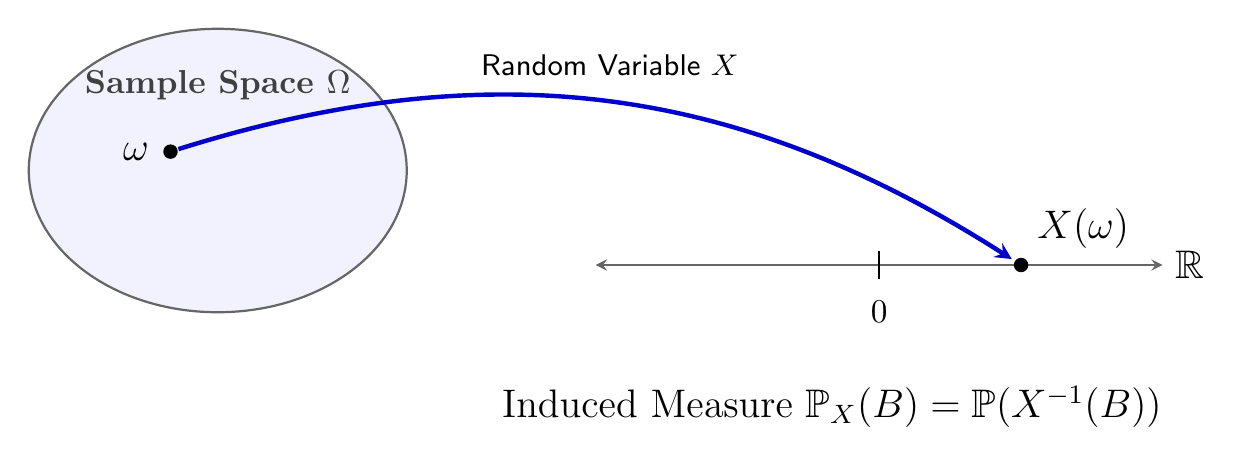
\begin{tikzpicture}[>=stealth, scale=1.2, transform shape]
    % 1. Probability Space (Ellipse)
    \draw[thick, fill=blue!5, draw=gray!80!black] (0,0) ellipse (2cm and 1.5cm);
    % Positioned clearly inside with breathing room
    \node[font=\bfseries, darkgray] at (0, 0.9) {Sample Space $\Omega$};
    
    % Point omega inside the sample space
    \coordinate (omega) at (-0.5, 0.2);
    \filldraw[black] (omega) circle (2pt);
    \node[left=3pt, font=\large] at (omega) {$\omega$};
    
    % 2. Real Number Line R
    \draw[thick, <->, gray!80!black] (4,-1) -- (10,-1) node[right, black, font=\large] {$\mathbb{R}$};
    
    % Crisp Tick Mark for 0
    \draw[thick] (7,-0.85) -- (7,-1.15) node[below=3pt] {$0$};
    
    % Point X(omega) on the real line
    \coordinate (Xomega) at (8.5, -1);
    \filldraw[black] (Xomega) circle (2pt);
    % Positioned above-right to completely clear the axis line and arrow
    \node[above right=2pt, font=\large] at (Xomega) {$X(\omega)$};
    
    % 3. Clean Mapping Arrow (Zero Collisions)
    % shorten filters keep the arrowhead cleanly separated from the dot and text
    \draw[->, ultra thick, blue!80!black, bend left=25, shorten <=3pt, shorten >=4pt] 
        (omega) to node[midway, above=4pt, black, font=\small\sffamily] {Random Variable $X$} (Xomega);
    
    % 4. Lower Formula / Induced Measure Block
    \node[font=\large] at (6.5, -2.5) {Induced Measure $\mathbb{P}_X(B) = \mathbb{P}(X^{-1}(B))$};
\end{tikzpicture}
\end{center}


\subsection{Heuristics and "Cheats"}
\begin{itemize}
    \item \textbf{LOTUS vs. Transformation:} If a question asks for the \textit{expected value} of a transformed variable (e.g., $\E[X^2]$), always use LOTUS. If the question asks for the \textit{probability} of a transformed variable (e.g., $\Prob(X^2 < 4)$), you must find the new CDF or integrate the original PDF over the transformed bounds.
    \item \textbf{Symmetry Shortcut:} For the standard normal distribution, utilize the symmetry property: $\Prob(Z < -z) = \Prob(Z > z) = 1 - \Prob(Z < z)$.
\end{itemize}

\subsection{Pitfalls and Fallacies}
\begin{itemize}
    \item \textbf{Jensen's Inequality Fallacy:} Assuming that $\E[g(X)] = g(\E[X])$. This is strictly false for non-linear functions. For example, $\E[X^2] \neq (\E[X])^2$.
    \item \textbf{The Point-Probability Trap:} For continuous distributions, $\Prob(X = c) = 0$. A common mistake is attempting to use the PDF value $f(c)$ as a probability. The PDF is a density, not a probability mass.
\end{itemize}

\newpage
\section{Part 5: Conceptual Synthesis and The "Big Picture"}

\subsection{Thematic Connections}
The central theme of this topic is \textbf{using measure theory to formalize randomness over continuous domains}. In discrete probability, we relied on combinatorics and counting finite sets. However, when dealing with time, space, or physical measurements, the sample space becomes uncountably infinite. The introduction of the Probability Density Function (PDF) unifies calculus and probability, allowing us to compute probabilities as areas under a curve (Lebesgue integrals) rather than sums of discrete masses.

\subsection{Forward and Backward Links}
\begin{itemize}
    \item \textbf{Backward Links:} This topic logically extends Riemann integration and the Fundamental Theorem of Calculus. It also builds upon discrete probability by acting as a limiting case (e.g., the Normal distribution is the continuous limit of the discrete Binomial distribution, as proven by the De Moivre-Laplace theorem).
    \item \textbf{Forward Links:} Understanding continuous distributions and their $\sigma$-algebras is the absolute bedrock for advanced Stochastic Calculus. The Normal distribution is the foundational building block for Brownian Motion (Wiener processes), which is essential for modeling continuous-time random walks in physics and finance.
\end{itemize}

\section{Part 6: Abstract Real-World Modeling (AI, ML, \& Quant Finance)}

\subsection{Concrete Scenarios}
\begin{enumerate}
    \item \textbf{Quantitative Finance (Black-Scholes Option Pricing):} The continuous normal distribution is used to model the logarithmic returns of stock prices. By assuming stock prices follow Geometric Brownian Motion, quantitative analysts use Ito's Lemma to derive the Black-Scholes partial differential equation for pricing European options.
    \item \textbf{Generative AI (Variational Autoencoders - VAEs):} In deep learning, VAEs generate new data (like images) by mapping inputs to a continuous latent space. This latent space is strictly modeled using multivariate Normal distributions. The network learns to minimize the Kullback-Leibler (KL) divergence between the encoded distribution and a standard normal prior.
\end{enumerate}

\subsection{Model Problem Setup: The Reparameterization Trick in VAEs}
In the context of Generative AI, let $\mathcal{X}$ be the space of observable data and $\mathcal{Z}$ be a continuous latent space. We define a prior over the latent variables $p(z) = \mathcal{N}(0, I)$. The true posterior $p(z|x)$ is intractable, so we approximate it with a parameterized neural network distribution $q_\phi(z|x)$, chosen to be a multivariate Gaussian with a diagonal covariance matrix:
\[ q_\phi(z|x) = \mathcal{N}(z; \mu_\phi(x), \text{diag}(\sigma_\phi^2(x))) \]
To optimize the Evidence Lower Bound (ELBO) loss function, we must compute gradients with respect to the network parameters $\phi$. However, sampling $z \sim q_\phi(z|x)$ is a stochastic process, which blocks deterministic backpropagation.

\textbf{The Mathematical Resolution:} We utilize the \textit{Reparameterization Trick}. We express the random variable $Z$ as a deterministic transformation of a parameter-free noise variable $\epsilon \sim \mathcal{N}(0, I)$:
\[ Z = \mu_\phi(x) + \sigma_\phi(x) \odot \epsilon \]
where $\odot$ denotes element-wise multiplication. This rigorous transformation isolates the randomness entirely within $\epsilon$. Because $\epsilon$ has no dependence on $\phi$, the gradient $\nabla_\phi$ can now flow deterministically through the continuous functions $\mu_\phi$ and $\sigma_\phi$, allowing the AI model to learn the parameters of the continuous normal distribution.

\newpage
\section{Part 7: Common Variations and Untested Concepts}

A critical concept in advanced probability not covered in the provided homework is the proof that the Normal density function actually integrates to 1 over the real line. This is known as the Gaussian Integral.

\textbf{Theorem:} $\int_{-\infty}^{\infty} e^{-x^2/2} \, dx = \sqrt{2\pi}$.

\textbf{Proof:}
Let $I = \int_{-\infty}^{\infty} e^{-x^2/2} \, dx$. Since the integrand is strictly positive, $I > 0$. We compute $I^2$ by multiplying the integral by itself, using a different dummy variable for the second integral:
\[ I^2 = \left( \int_{-\infty}^{\infty} e^{-x^2/2} \, dx \right) \left( \int_{-\infty}^{\infty} e^{-y^2/2} \, dy \right) \]
By Fubini's Theorem, we can combine this into a double integral over $\R^2$:
\[ I^2 = \int_{-\infty}^{\infty} \int_{-\infty}^{\infty} e^{-(x^2 + y^2)/2} \, dx \, dy \]
We transform the coordinates from Cartesian $(x,y)$ to polar $(r, \theta)$, where $x^2 + y^2 = r^2$ and the differential area element $dx \, dy$ becomes $r \, dr \, d\theta$. The limits of integration become $r \in [0, \infty)$ and $\theta \in [0, 2\pi]$:
\[ I^2 = \int_{0}^{2\pi} \int_{0}^{\infty} e^{-r^2/2} r \, dr \, d\theta \]
The inner integral can be solved using u-substitution. Let $u = r^2/2$, then $du = r \, dr$:
\[ \int_{0}^{\infty} e^{-r^2/2} r \, dr = \int_{0}^{\infty} e^{-u} \, du = \left[ -e^{-u} \right]_{0}^{\infty} = 0 - (-1) = 1 \]
Now, evaluate the outer integral:
\[ I^2 = \int_{0}^{2\pi} 1 \, d\theta = 2\pi \]
Taking the positive square root yields $I = \sqrt{2\pi}$. Therefore, dividing the integrand by $\sqrt{2\pi}$ ensures the total probability measure is exactly 1. $\blacksquare$

\newpage
\section{Part 8: Advanced Diagnostic Testing: "Find the Flaw"}

Below are five advanced proofs containing a single, subtle logical or mathematical flaw. 

\subsection{Problem 1: Expectation of an Inverse}
\textbf{Problem:} Let $X \sim \mathcal{N}(0,1)$. Prove that the expectation of the inverse, $\E[1/X]$, is exactly $0$. \\
\textbf{Flawed Proof:} By the Law of the Unconscious Statistician (LOTUS), we have:
\[ \E\left[\frac{1}{X}\right] = \int_{-\infty}^{\infty} \frac{1}{x} \frac{1}{\sqrt{2\pi}} e^{-x^2/2} \, dx \]
Let $f(x) = \frac{1}{x} e^{-x^2/2}$. Notice that $f(-x) = -f(x)$, meaning the integrand is an odd function. The integral of an odd function over a symmetric domain $(-\infty, \infty)$ is always $0$. Therefore, $\E[1/X] = 0$. $\blacksquare$

\subsection{Problem 2: Transformation of Variables}
\textbf{Problem:} Let $X \sim \mathcal{U}(-1, 1)$. Find the probability density function of $Y = X^2$. \\
\textbf{Flawed Proof:} We use the transformation method. The relationship is $y = x^2$, which implies $x = \sqrt{y}$. The derivative is $\frac{dx}{dy} = \frac{1}{2\sqrt{y}}$. The PDF of $X$ is $f_X(x) = \frac{1}{2}$ for $x \in [-1, 1]$. Using the transformation formula $f_Y(y) = f_X(x) \left| \frac{dx}{dy} \right|$, we get:
\[ f_Y(y) = \frac{1}{2} \left| \frac{1}{2\sqrt{y}} \right| = \frac{1}{4\sqrt{y}} \quad \text{for } y \in (0, 1] \]
Thus, the PDF of $Y$ is $f_Y(y) = \frac{1}{4\sqrt{y}}$. $\blacksquare$

\subsection{Problem 3: Scaling Variance}
\textbf{Problem:} Let $X \sim \mathcal{N}(\mu, \sigma^2)$. Prove that the variance of $2X$ is $2\sigma^2$. \\
\textbf{Flawed Proof:} Variance is a measure of spread or dispersion of a random variable. If we scale a random variable by a constant factor of $c$, the spread scales proportionally by that exact same factor. Therefore, the general rule is $\text{Var}(cX) = c \text{Var}(X)$. Letting $c = 2$, we get $\text{Var}(2X) = 2\text{Var}(X) = 2\sigma^2$. $\blacksquare$

\subsection{Problem 4: Probability of Rationals}
\textbf{Problem:} Let $X \sim \mathcal{U}(0,1)$. Find the probability that $X$ is a rational number. \\
\textbf{Flawed Proof:} The set of rational numbers $\Q$ is dense in the real numbers $\R$. This means that between any two real numbers, there exists a rational number. Because the rationals are ubiquitous and infinitely packed throughout the interval $[0,1]$, the probability of selecting a rational number is certain. Thus, $\Prob(X \in \Q) = 1$. $\blacksquare$

\subsection{Problem 5: Maximizing the Normal Density}
\textbf{Problem:} Find the value of $x$ that maximizes the standard normal density function $f(x) = \frac{1}{\sqrt{2\pi}} e^{-x^2/2}$. \\
\textbf{Flawed Proof:} To maximize $f(x)$, we can equivalently maximize its natural logarithm, since $\ln(x)$ is a strictly increasing function.
\[ \ln f(x) = \ln\left(\frac{1}{\sqrt{2\pi}}\right) - \frac{x^2}{2} \]
To maximize this expression, we must maximize the term $-\frac{x^2}{2}$. Since $x^2 \ge 0$, the term $-\frac{x^2}{2}$ grows infinitely large as $x \to \infty$. Therefore, the maximum occurs at $x = \infty$. $\blacksquare$

\vspace{2em}
\hrule
\vspace{1em}
\subsection*{Solution Key: Resolution of Flaws}
\textbf{Resolution 1:} The flaw is assuming the integral converges. The integral $\int_{-\infty}^{\infty} \frac{1}{x} e^{-x^2/2} \, dx$ is improper and has a non-integrable singularity at $x=0$. For an expectation to exist, the integral of the absolute value must be finite ($\int |x|^{-1} e^{-x^2/2} \, dx < \infty$), which diverges. Thus, $\E[1/X]$ is undefined. \\
\textbf{Resolution 2:} The transformation $y = x^2$ is not one-to-one on $[-1, 1]$. We must account for both branches: $x_1 = \sqrt{y}$ and $x_2 = -\sqrt{y}$. The correct PDF requires summing over both branches: $f_Y(y) = f_X(\sqrt{y})\left|\frac{dx_1}{dy}\right| + f_X(-\sqrt{y})\left|\frac{dx_2}{dy}\right| = \frac{1}{4\sqrt{y}} + \frac{1}{4\sqrt{y}} = \frac{1}{2\sqrt{y}}$. \\
\textbf{Resolution 3:} Variance does not scale linearly; it scales quadratically. Because variance is defined as the expected value of squared deviations, $\text{Var}(cX) = c^2 \text{Var}(X)$. The correct variance is $4\sigma^2$. \\
\textbf{Resolution 4:} While $\Q$ is dense in $\R$, it is a countably infinite set. In measure theory, the Lebesgue measure (and thus the uniform probability measure) of any countable set of points is exactly $0$. Thus $\Prob(X \in \Q) = 0$. \\
\textbf{Resolution 5:} The flaw is an algebraic sign error. To maximize $\ln f(x) = C - \frac{x^2}{2}$, we must \textit{minimize} the subtracted term $\frac{x^2}{2}$. The minimum of $x^2/2$ occurs at $x=0$, which correctly corresponds to the peak of the bell curve.

\end{document}